\subsection{Forum}\label{forum}
Te vinden op \drupalpath{forum}.

\subsubsection{Aanmaken forumcategorieen}\label{forumcategorieen}
Op \drupalpath{admin/structure/taxonomy/forums} zijn forumonderwerpen aan te maken. Dit zijn de onderwerpen op het hoogste niveau binnen het forum. Voor de onderwerpen worden taxonomietermen gebruik.

\subsubsection{Aanmaken forumonderwerpen}\label{forumonderwerpen}
Het aanmaken van een nieuw forumonderwerp doe je door op de knop \emph{Forumonderwerp toevoegen} te drukken. Hierna volgt een itembewerkpagina waar je het onderwerp kan aanmaken. Selecteer een forumcategorie (Forums) om het onderwerp in een van de categorieen te plaatsen. Maak je een nieuw onderwerp aan binnen een categorie zal deze automatisch geselecteerd zijn.

\begin{center}
	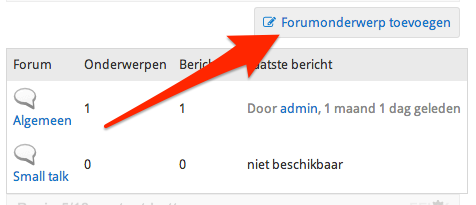
\includegraphics[width=\textwidth]{img/forumonderwerp.png}
\end{center}